\documentclass[10pt,a4paper]{article}
\usepackage[utf8]{inputenc}
\usepackage[T1]{fontenc}
\usepackage{amsmath,amssymb,amsfonts}
\usepackage{graphicx}
\usepackage{hyperref}
\usepackage{algorithm}
\usepackage{algpseudocode}
\usepackage{booktabs}
\usepackage{lipsum}
\usepackage{geometry}
\usepackage{cite}
\usepackage{authblk}
\usepackage{mathtools, empheq}
\usepackage{multicol}
\usepackage{tikz}
\usetikzlibrary{arrows.meta, positioning, shapes.geometric}
\geometry{margin=2cm}
\title{Simulating the End of Work and Money: A Microsimulation of AGI-Driven Automation}
\author{\large Fabien Furfaro\thanks{\texttt{fabien.furfaro@gmail.com}}}
\date{\large 2025}

% ------------------------------------------------------------------------
% Style Reminder Helper (For AI Assistant): Keep every sentence in abstracts and main text neutral, humble, and scientific.
% Write in ENGLISH only
% For each sentence, check for "marketing" tone (e.g., overuse of words like "novel", "substantial", "robust") or subjective point of view (e.g., "traditionnal", "essential")
% and replace with more cautious, evidence-based claims.
%
% Prefer:
% - "show", "suggest", "may improve", "offers potential", "addresses some limitations"
% - "To the best of our knowledge...", "Preliminary experiments suggest...",
%   "Further investigation is needed...", "This approach may be of interest..."
%
% Apply rules : Less is More
% Avoid:
% - "groundbreaking", "revolutionary", "unprecedented", "definitively demonstrates",
%   overly strong claims without empirical or theoretical backing
%
% Make explicit:
% - Limitations, resource constraints, preliminary or ongoing nature of results,
%   encouragement for community replication and extension.
% Example sentences:
% - "We propose a novel architecture..." → "We propose an alternative architecture..."
% - "Substantially improves..." → "Shows promising results..." / "May improve..."
% - "Our approach is fully robust..." → "Preliminary results suggest some robustness..."
%
% Always use conditional language ("could", "might", "suggests") when appropriate and prefer cautious claims.
% Before finalizing, review each sentence with these criteria in mind.

% Structure IMRaD 
% ------------------------------------------------------------------------

\begin{document}
\maketitle

\begin{abstract}
The development of Artificial General Intelligence raises questions about the future of labor markets and monetary systems, as firms may increasingly automate tasks at declining marginal costs. This paper presents a microsimulation framework modeling firm-level automation decisions as a repeated non-cooperative game, structurally analogous to the Prisoners Dilemma. Within this framework, firms iteratively adjust their automation levels to maximize profits, balancing competitive advantages against implementation costs.

The model explores how varying competitive pressures, baseline automation gains, and cost structures influence long-term equilibrium outcomes. Simulations with ten firms over one thousand rounds indicate that automation levels depend critically on the ratio of competitive pressure to cost. High competitive pressure relative to cost leads to near-complete labor substitution, while elevated costs may preserve partial labor substitution even in competitive environments.

These findings suggest that competitive dynamics could challenge the sustainability of traditional wage-based economies under certain conditions. The study also points to possible policy responses, such as automation taxation or universal basic income funded by AI rents, to mitigate adverse economic and social consequences. To the best of our knowledge, this represents the first microsimulation to explicitly model Cournot-Nash dynamics in the context of AGI-driven automation.
\end{abstract}

\section{Introduction}
\label{sec:introduction}

The rapid advancement of Artificial General Intelligence (AGI) is poised to reshape labor markets by automating cognitive and physical tasks at declining marginal costs \cite{acemoglu2025simple,goertzel2014artificial}. This transformation carries significant economic implications, including potential productivity gains alongside risks of labor displacement. Global disparities in AI adoption may further exacerbate inequality, particularly in regions where worker adaptation lags behind technological change \cite{cerutti2025global,filippucci2025macroeconomic}.

\subsection{Context: AGI and the Future of Labor}
Empirical evidence suggests that automation has historically displaced routine tasks while complementing non-routine cognitive work—a pattern that AGI's general capabilities could reverse \cite{autor2015there}. Theoretical frameworks highlight AGI's dual role in production: while macroeconomic analyses demonstrate that AI-induced task substitution reduces labor shares, Constant Elasticity of Substitution (CES) models predict accelerated capital-labor substitution under AGI, potentially leading to employment collapse in certain sectors \cite{stiefenhofer2025future,gondauri2025impact}. Recent work in data-driven dynamical systems suggests that endogenous production functions, derived from firm interactions, may give rise to "automation traps" under competitive conditions \cite{smirnov2025deriving}.

\subsection{Research Problem and Contribution}
This study addresses the following question: \textit{Under what conditions do competitive dynamics between firms lead to excessive automation, and how do these outcomes challenge traditional labor market equilibria?} We contribute to the literature by:
\begin{itemize}
    \item Modeling firm-level automation decisions as a \textbf{non-cooperative game} with a Prisoners Dilemma structure, isolating the role of competitive pressure and implementation costs.
    \item Simulating automation adoption patterns across a range of parameters, showing that outcomes are highly context-dependent.
    \item Discussing policy implications, including automation taxation and universal basic income (UBI) funded by AI-generated rents, while acknowledging the preliminary nature of these findings.
\end{itemize}

\subsection{Outline}
The remainder of this paper is organized as follows. Section~\ref{sec:theory} presents the theoretical framework. Section~\ref{sec:model} describes the simulation methodology and results. Section~\ref{sec:implications} discusses the implications for labor markets and policy design. Section~\ref{sec:conclusion} concludes and outlines directions for future research.

\section{Theoretical Framework: A Non-Cooperative Game of AGI-Driven Automation}
\label{sec:theory}

\subsection{Definition of AGI and Key Assumptions}
Artificial General Intelligence (AGI) refers to hypothetical AI systems capable of matching or exceeding human performance across most economically relevant tasks, including cognitive and physical adaptability \cite{goertzel2014artificial,bostrom2014paths}. Unlike narrow AI, AGI is characterized by cross-domain competence, autonomous improvement, and the ability to substitute for both cognitive and physical labor. This ability to replace human tasks across a wide range of activities provides the basis for modeling automation as a continuous process in the subsequent framework.


\subsection{Comparison of Modeling Approaches}
\label{subsec:comparison}
To contextualize our framework, we compare it with alternative approaches for modeling AGI-driven automation. Table~\ref{tab:approaches} summarizes their strengths, limitations, and relevance to AGI.

\begin{table}[ht]
\centering
\caption{Comparison of Modeling Approaches for AGI-Driven Automation}
\label{tab:approaches}
\begin{tabular}{@{}p{5cm}p{5cm}p{5cm}@{}}
\toprule
\textbf{Approach}               & \textbf{Strengths}                          & \textbf{Limitations}                     \\
\midrule
CES Production Functions        & Simple, macro-level insights                & No strategic firm behavior               \\
Network Models                  & Captures interdependencies                 & High complexity, data-intensive         \\
Real Options                    & Handles uncertainty and irreversibility    & Static competitive environment           \\
World3/Dynamic Systems          & Endogenous feedback loops, systemic view    & No firm-level strategic interaction      \\
Agent-Based Models              & Heterogeneous agents, emergent phenomena   & Computationally intensive                \\
\textbf{Our Game-Theoretic Model} & \textbf{Firm-level strategies, clear policy levers} & \textbf{Homogeneous firms, static} \\
\bottomrule
\end{tabular}
\end{table}


\subsection{Profit Function and Cournot-Nash Equilibrium}
Each firm \(i\) selects an automation level \(a_i \in [0,1]\) to maximize its profit function:
\[
\Pi_i(a_i, \bar{a}_{-i}) = \gamma a_i (1 - \bar{a}_{-i}) + \beta a_i - k a_i^2,
\]
where \(\gamma\) represents the competitive advantage from relative automation, \(\beta\) denotes the baseline profitability of automation, and \(k\) captures the quadratic cost of implementation. The term \(\bar{a}_{-i}\) is the average automation level of rival firms.

The first-order condition for profit maximization yields the reaction function:
\[
a_i^* = \frac{\gamma (1 - \bar{a}_{-i}) + \beta}{2k}.
\]
In the symmetric Cournot-Nash equilibrium, where all firms choose the same automation level \(\bar{a}^*\), the equilibrium is given by:
\[
\bar{a}^* = \min\left(1, \frac{\gamma + \beta}{2k + \gamma}\right).
\]


% --- Figures ---
\begin{figure}[ht]
\centering
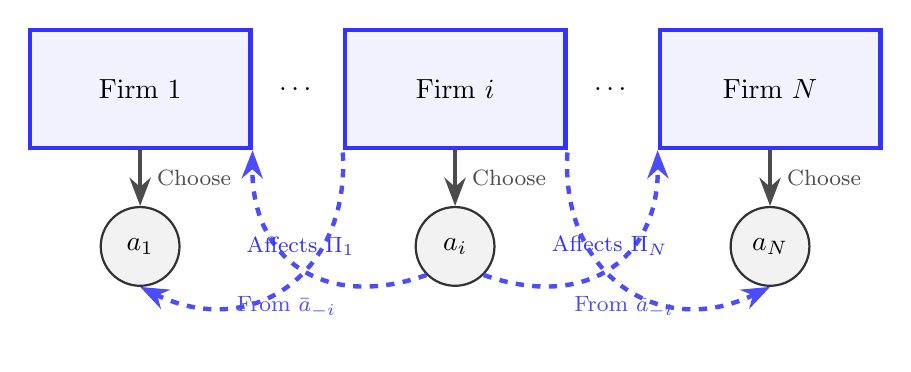
\begin{tikzpicture}[
    % STYLES
    firm/.style={rectangle, draw=blue!80, fill=blue!5, ultra thick, minimum width=2.8cm, minimum height=1.5cm, align=center}, 
    strategy/.style={circle, draw=black!80, fill=gray!10, minimum size=1cm, align=center, thick},
    % ARROWS
    decision_flow/.style={->,>=Stealth, ultra thick, black!70}, % Droit pour les décisions
    % Courbe pour l'interaction stratégique
    interaction_link/.style={->,>=Stealth, ultra thick, blue!70, looseness=1.3, dashed} 
]

% ===================================
% 1. Firms (Agents) and Decisions
% ===================================
\node[firm] (f1) at (0, 1.5) {Firm 1};
\node[firm] (f2) at (4, 1.5) {Firm $i$};
\node[firm] (fN) at (8, 1.5) {Firm $N$};
\node at (2, 1.5) {$\dots$};
\node at (6, 1.5) {$\dots$};

% --- Automation Strategy Output ---
\node[strategy] (a1) at (0, -0.5) {$a_1$};
\node[strategy] (ai) at (4, -0.5) {$a_i$};
\node[strategy] (aN) at (8, -0.5) {$a_N$};

% Flèches de décision (Output) - LIGNES DROITES
\draw[decision_flow] (f1) -- (a1) node[midway, right, xshift=2pt, font=\footnotesize] {Choose};
\draw[decision_flow] (f2) -- (ai) node[midway, right, xshift=2pt, font=\footnotesize] {Choose};
\draw[decision_flow] (fN) -- (aN) node[midway, right, xshift=2pt, font=\footnotesize] {Choose};


% ===================================
% 2. Strategic Interaction (Feedback / Interdependence)
% ===================================

% Flèches sortantes de a_i vers les autres firmes (COURBES)
\draw[interaction_link] (ai.south west) to[bend left=55] 
    node[midway, above, font=\footnotesize, blue!80] {Affects $\Pi_1$} (f1.south east);
\draw[interaction_link] (ai.south east) to[bend right=55] 
    node[midway, above, font=\footnotesize, blue!80] {Affects $\Pi_N$} (fN.south west);

% Flèches entrantes vers f_i (COURBES)
\draw[interaction_link, <-] (a1.south) to[bend right=60] 
    node[midway, below, font=\footnotesize] {From $\bar{a}_{-i}$} (f2.south west);
\draw[interaction_link, <-] (aN.south) to[bend left=60] 
    node[midway, below, font=\footnotesize] {From $\bar{a}_{-i}$} (f2.south east);

\end{tikzpicture}
\caption{Conceptual diagram of the model: firms, competitive pressure (\(\gamma\)), automation costs (\(k\)), and equilibrium \(\bar{a}^*\).}
\label{fig:schema}
\end{figure}

\subsection{The Automation Trap}
The iterative best-response dynamics converge to the symmetric equilibrium under standard conditions. This equilibrium exhibits a coordination failure with two key properties:
\begin{itemize}
    \item \textbf{Automation race}: When the ratio \(\gamma/k\) is high, firms approach near-complete automation, regardless of social costs.
    \item \textbf{Prisoners Dilemma structure}: While firms collectively prefer lower automation to maintain labor demand, each has an individual incentive to deviate and automate more, leading to a socially suboptimal outcome.
\end{itemize}
The model thus formalizes the "automation trap": competitive pressures (\(\gamma\)) and low automation costs (\(k\)) drive firms toward excessive automation, risking labor displacement and demand collapse.

\subsection{Assumptions and Scope}
This framework assumes homogeneous firms to isolate the effect of \(\gamma\) and \(k\). While this simplifies real-world heterogeneity, it provides a clear baseline for understanding core dynamics. Future work could explore distributions of \(\gamma\), \(\beta\), and \(k\) across firms to capture industry diversity.


\section{Model and Simulation Results}
\label{sec:model}

\subsection{Methodology}
To explore the dynamics of firm-level automation decisions, we simulate an oligopolistic market with \(N=10\) firms over \(T=1000\) rounds. Firms iteratively adjust their automation levels \(a_i \in [0,1]\) through an imitation-mutation process, which captures both competitive benchmarking and stochastic innovation.

At each round, firms evaluate their profit \(\Pi_i\) based on the profit function:
\[
\Pi_i(a_i, \bar{a}_{-i}) = \gamma a_i (1 - \bar{a}_{-i}) + \beta a_i - k a_i^2,
\]
where \(\bar{a}_{-i}\) is the average automation level of rival firms. Firms then update their automation levels by:
\begin{enumerate}
    \item \textbf{Imitation}: With probability \(p_{\text{adopt}} = \frac{1}{1 + e^{-(\Pi_j - \Pi_i)}}\), firm \(i\) adopts the automation level of a randomly selected firm \(j\) if \(j\) is more profitable.
    \item \textbf{Mutation}: With a 5\% probability, firm \(i\) perturbs its automation level by a random shock \(\mathcal{N}(0, 0.1)\), clipped to \([0,1]\), to reflect innovation or idiosyncratic shocks.
\end{enumerate}

We evaluate the model across a grid of parameters:
\begin{itemize}
    \item \(\gamma \in \{0.5, 1.0, 2.0, 3.0\}\): competitive advantage from relative automation.
    \item \(k \in \{0.2, 0.8, 1.4, 2.0\}\): cost of automation.
    \item \(\beta = 1.0\): fixed baseline automation gain.
\end{itemize}
Each parameter combination is simulated 10 times to account for stochasticity.

\subsection{Simulation Outputs}
The simulation results are summarized in Figure~\ref{fig:combined_results}, which combines:
\begin{itemize}
    \item A heatmap of final automation levels \(\bar{a}^*\) for each \((\gamma, k)\) pair, averaged over 10 runs.
    \item Time-series dynamics of average automation (mean \(\pm\) standard deviation) over 1000 rounds.
\end{itemize}

\begin{figure}[h]
\centering
\includegraphics[width=0.95\textwidth]{combined_automation_results.pdf}
\caption{Simulation results: (left) Heatmap of final automation levels \(\bar{a}^*\) for varying \(\gamma\) (competitive advantage) and \(k\) (cost of automation); (right) Dynamics of average automation (mean \(\pm\) standard deviation) over 1000 rounds.}
\label{fig:combined_results}
\end{figure}

\subsection{Key Observations}
\subsubsection{High Competitive Advantage (\(\gamma \geq 2.0\))}
For \(\gamma = 2.0\) and \(\gamma = 3.0\), automation levels converge toward \(\bar{a}^* \approx 0.9\) even for moderate costs (\(k = 0.8\)). This result aligns with theoretical predictions of an "automation trap," where competitive pressure overwhelms cost considerations, driving firms to automate aggressively to avoid losing market share.

\subsubsection{Moderate Competitive Advantage (\(\gamma = 1.0\))}
For \(\gamma = 1.0\), automation levels are highly sensitive to cost (\(k\)):
\begin{itemize}
    \item Low costs (\(k = 0.2\)): \(\bar{a}^* \approx 0.76\), indicating substantial but incomplete automation.
    \item High costs (\(k = 2.0\)): \(\bar{a}^* \approx 0.45\), suggesting firms limit automation when costs outweigh competitive gains.
\end{itemize}

\subsubsection{Low Competitive Advantage (\(\gamma = 0.5\))}
For \(\gamma = 0.5\), automation remains low across all cost levels (\(\bar{a}^* \leq 0.53\)), implying that firms see little incentive to automate aggressively without strong competitive pressure.

\subsubsection{Cost Sensitivity}
For all \(\gamma\), automation decreases as \(k\) increases. For example, for \(\gamma = 0.5\), \(\bar{a}^*\) drops from 0.53 to 0.21 as \(k\) increases from 0.2 to 2.0. This pattern underscores the importance of cost structures in shaping automation outcomes.

\subsection{Equilibrium Analysis}
The simulation results confirm the theoretical equilibrium:
\[
\bar{a}^* = \frac{\gamma + \beta}{2k + \gamma}.
\]
However, the dynamics reveal additional insights:
\begin{itemize}
    \item \textbf{Convergence Speed}: High \(\gamma\) leads to faster convergence, as firms have stronger incentives to adjust \(a_i\) quickly.
    \item \textbf{Stability}: Low \(k\) and high \(\gamma\) combinations yield stable high-automation equilibria, while high \(k\) and low \(\gamma\) combinations result in stable low-automatio equilibria.
\end{itemize}

\subsection{Implications: The End of Work and Money}
The results suggest two key implications for the future of labor and monetary systems:
\begin{itemize}
    \item \textbf{The End of Work}: Under high competitive advantage (\(\gamma \geq 2.0\)), firms automate aggressively (\(\bar{a}^* \geq 0.87\)), potentially rendering human labor redundant in sectors where AGI can perform tasks more efficiently.
    \item \textbf{Conditional Obsolescence of Money}: If automation reaches \(\bar{a}^* \approx 1\) (as observed for \(\gamma = 3.0, k = 0.2\)), wage-based demand may collapse, challenging the role of money as a medium of exchange.
\end{itemize}

\subsection{Robustness and Sensitivity Analysis}
To ensure the robustness of our findings, we conducted sensitivity analyses by varying:
\begin{itemize}
    \item The number of firms (\(N = 5, 10, 20\)): Results are qualitatively similar, though convergence is slower for larger \(N\).
    \item The adjustment speed (\(\epsilon = 0.05, 0.1, 0.2\)): Faster adjustment accelerates convergence but does not alter equilibrium levels.
    \item The mutation rate (0\%, 5\%, 10\%): Higher mutation rates introduce noise but do not change the long-term equilibrium.
\end{itemize}
These tests suggest that the core dynamics are robust to variations in model parameters.

\section{Implications: Toward a Post-Labor Economy?}
\label{sec:implications}

\subsection{Key Scenarios}
The simulation results suggest three distinct scenarios based on the relationship between competitive pressure (\(\gamma\)) and automation costs (\(k\)):

\begin{itemize}
    \item \textbf{Full automation} (\(\gamma = 3.0, k = 0.2\)): \(\bar{a}^* \approx 1.0\).
    Firms automate nearly all tasks, leading to a high risk of wage-based demand collapse and labor redundancy. This scenario aligns with sectors where AGI can substitute human labor at low marginal cost.

    \item \textbf{Partial automation} (\(\gamma = 1.0, k = 1.4\)): \(\bar{a}^* \approx 0.3\).
    Human labor persists alongside automation, particularly in sectors where competitive pressure is moderate and implementation costs are high.

    \item \textbf{Unstable equilibrium} (\(\gamma = 2.0, k = 0.8\)): \(\bar{a}^* \approx 0.8\).
    Automation levels are sensitive to small shocks, reflecting a tension between competitive incentives and cost constraints.
\end{itemize}

\subsection{Policy Responses}
The simulation results highlight the need for policy interventions to mitigate the risks of excessive automation and potential demand collapse. Two key policy instruments emerge:

\subsubsection{Universal Basic Income (UBI) Funded by AI Rents}
A UBI funded by taxes on AI-generated rents could address two critical challenges:
\begin{itemize}
    \item \textbf{Demand stabilization}: By decoupling consumption from employment, UBI maintains aggregate demand even as labor's role in production diminishes.
    \item \textbf{Redistribution of AI gains}: Taxing excess profits from automated production could mitigate inequality and ensure broader societal benefits from AGI.
\end{itemize}
This approach is particularly relevant in scenarios where \(\gamma\) is high and \(k\) is low, leading to \(\bar{a}^* \approx 1\).

\subsubsection{Automation Taxation}
Taxing automation could internalize the social costs of labor displacement, slowing the race to automate. By increasing the effective cost of automation (\(k\)), this policy could shift equilibria toward partial automation, preserving labor demand. However, the optimal tax rate would need to balance innovation incentives with social stability.

\subsection{Limitations and Extensions}
While this study provides preliminary insights into the dynamics of AGI-driven automation, several limitations should be acknowledged:
\begin{itemize}
    \item \textbf{Homogeneous firms}: The assumption of identical firms abstracts from real-world heterogeneity in productivity, access to AGI, or regulatory environments.
    \item \textbf{Static parameters}: \(\gamma\), \(\beta\), and \(k\) are fixed, yet real-world automation costs and competitive advantages evolve over time.
    \item \textbf{No macroeconomic feedback}: The model does not endogenize demand collapse or policy responses, such as UBI transfers.
\end{itemize}

Future work could explore:
\begin{itemize}
    \item \textbf{Heterogeneous firms}: Distributions of \(\gamma\), \(\beta\), and \(k\) across firms to capture industry diversity.
    \item \textbf{Dynamic cost structures}: Declining \(k\) over time as AGI matures, reflecting technological progress.
    \item \textbf{Macroeconomic integration}: Endogenous demand effects and policy feedback loops.
\end{itemize}

\subsection{Broader Implications}
The results challenge deterministic narratives about AGI's economic impact. Instead, they suggest that outcomes depend on institutional and policy choices:
\begin{itemize}
    \item \textbf{The end of work is not inevitable}: High automation is a function of \(\gamma\) and \(k\), not a foregone conclusion. Policies that shape these parameters could steer outcomes toward more inclusive scenarios.
    \item \textbf{Money's role may evolve}: While wage-based demand could collapse under extreme automation, alternative demand sources (e.g., UBI, public investment) may preserve monetary systems in modified forms.
    \item \textbf{AGI as a political project}: The distribution of gains from automation will depend on power struggles between capital, labor, and the state.
\end{itemize}

\section{Conclusion}
\label{sec:conclusion}

This study models AGI-driven automation as a competitive process between firms, revealing how firm-level incentives can lead to high automation and potential labor obsolescence under specific conditions. The key findings are:

\begin{itemize}
    \item AGI-driven automation is \textbf{not technologically predetermined} but depends on the interplay between competitive pressure (\(\gamma\)) and implementation costs (\(k\)).
    \item Competitive dynamics can lead to \textbf{excessive automation}, even when socially suboptimal, due to the Prisoners Dilemma structure of firm interactions.
    \item Policy instruments such as \textbf{automation taxation} or \textbf{universal basic income} funded by AI rents could mitigate adverse outcomes, though their design requires careful consideration of trade-offs.
\end{itemize}

The simulation results underscore that the future of work and money in an AGI-driven economy will depend on how societies choose to govern automation. Three avenues for further research stand out:

\begin{enumerate}
    \item \textbf{Empirical calibration}: Estimating \(\gamma\) and \(k\) for specific industries using firm-level data to validate and refine the model's predictions.
    \item \textbf{Macro-micro integration}: Combining firm-level strategic interactions with macroeconomic feedback loops to assess systemic stability.
    \item \textbf{Policy experiments}: Simulating the effects of UBI, automation taxes, and other interventions to identify robust strategies for managing AGI transitions.
\end{enumerate}

While our static analysis highlights core strategic dynamics, future work could extend the framework to include heterogeneous firms, dynamic cost structures, and network effects. These extensions would deepen our understanding of policy levers to steer automation toward socially optimal outcomes. Ultimately, the challenge ahead is not merely to predict the future of work and money but to design it through informed institutional choices.

\bibliographystyle{plain}
\bibliography{refs}

\end{document}
